\documentclass[11pt]{article}
\usepackage{mathblatt}


\begin{document}
\pfheftstil
\pfheftkopf{Flaechen}{P10}
\pfrueckblick
\begin{pfaufg}{}{1.}{}
Schreib kürzer: a + a + a; a · a; 2 · a + 2 · b.
\fusshilfe{\mbox{1:~3a; a²; 2(a + b)}}
\end{pfaufg}
\begin{pfaufg}{}{2.}{}
Ergänze die Tabelle Figur | Formel.
\par\smallskip\noindent \begingroup\renewcommand{\arraystretch}{1.3}\begin{tabular}{|c|c|}\hline \textbf{Figur} & \textbf{Formel} \\ \hline A & \rule{0pt}{3ex}\hspace{1.6cm} \\ \hline A & \rule{0pt}{3ex}\hspace{1.6cm} \\ \hline A & \rule{0pt}{3ex}\hspace{1.6cm} \\ \hline A & \rule{0pt}{3ex}\hspace{1.6cm} \\ \hline A & \rule{0pt}{3ex}\hspace{1.6cm} \\ \hline\end{tabular}\endgroup\par
\fusshilfe{\mbox{2:~A = e · f : 2}}
\end{pfaufg}
\begin{pfaufg}{}{3.}{}
Zwei Halbkreise mit 5 m Durchmesser ergeben zusammen einen Kreis. Gib seinen Radius an. Ein Trapez hat unten 20 m, oben 12 m; es ist symmetrisch. Wie weit steht die untere Seite auf jeder Seite über?
\rechenplatz{1}
\fusshilfe{\mbox{3:~r = 2,5 m; (20 $-$ 12) : 2 = 4 m}}
\end{pfaufg}
\pfstufekopf[sformelodertermzurfig]{Formel oder Term zur Figur}{in 3 der letzten 5 Prüfungen}
\pfgruppe{}
\begin{pfaufg}{}{4.}{}
Ein Garten bekommt einen Zaun. Kreuze an, ob du dafür die Fläche oder den Umfang brauchst. 
\pfkreuzzeile{Fläche}\pfkreuzzeile{Umfang}
\fusshilfe{\mbox{4:~Umfang}}
\end{pfaufg}
\begin{pfaufg}{}{5.}{}
Die Figur zeigt ein Dreieck mit der Grundseite $g$. Zeichne die Höhe zu $g$ ein und markiere den rechten Winkel.
\par\smallskip\noindent \dreieck{(0,0)}{(5,0)}{(2,3)}{}{}{g}{}{}{}\par
\rechenplatz{1}
\fusshilfe{\mbox{5:~Strecke von C senkrecht auf AB}}
\end{pfaufg}
\pfgruppe{}
\begin{pfaufg}{}{6.}{}
Ein Rechteck hat die Länge $a = 8$ cm und die Breite $b = 3$ cm. Berechne die Fläche und den Umfang des Rechtecks.
\par\noindent A = \leerfeld[cm²] , u = \leerfeld[cm] \par
\fusshilfe{\mbox{6:~$22$ cm}}
\end{pfaufg}
\begin{pfaufg}{}{7.}{}
Ein Dreieck hat die Grundseite $g = 8$ cm und die Höhe $h = 7$ cm. Berechne die Fläche des Dreiecks.
\par\noindent A = \leerfeld[cm²] \par
\fusshilfe{\mbox{7:~$28$ cm²}}
\end{pfaufg}
\begin{pfaufg}{}{8.}{}
Ein Dreieck hat den Umfang $u = 3 \cdot k$. Zeichne das Dreieck und beschrifte die Seiten.
\par\smallskip\noindent \rechenplatz[halb]{4}\par
\rechenplatz{1}
\fusshilfe{\mbox{8:~gleichseitiges Dreieck mit drei Seiten $k$}}
\end{pfaufg}
\pfgruppe{}
\begin{pfaufg}{P10 ’19}{9.}{1 BE}
Gib eine Gleichung für den Flächeninhalt A der gesamten Fläche an.
\par\smallskip\noindent 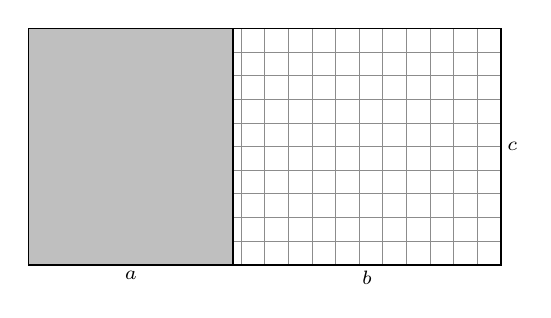
\begin{tikzpicture}[x=1.000cm,y=1.000cm,line width=0.6pt,baseline=(current bounding box.north)]\fill[black!25] (0.000,0.000) -- (2.600,0.000) -- (2.600,3.000) -- (0.000,3.000) -- cycle;\begin{scope}\clip (2.600,0.000) -- (6.000,0.000) -- (6.000,3.000) -- (2.600,3.000) -- cycle;\draw[black!45,line width=0.3pt,step=0.300] (-10,-10) grid (20,20);\end{scope}\draw (0.000,0.000) -- (6.000,0.000) -- (6.000,3.000) -- (0.000,3.000) -- cycle;\draw[] (2.600,0.000) -- (2.600,3.000);\node[font=\scriptsize,anchor=north,inner sep=2pt] at (1.300,0.000) {$a$};\node[font=\scriptsize,anchor=north,inner sep=2pt] at (4.300,0.000) {$b$};\node[font=\scriptsize,anchor=west,inner sep=2pt] at (6.000,1.500) {$c$};\end{tikzpicture}\par
\rechenplatz{1}
\fusshilfe{\mbox{9:~A = (a + b) · c}}
\end{pfaufg}
\begin{pfaufg}{P10 ’22}{10.}{1 BE}
Gib eine Gleichung für den Flächeninhalt A des Dreiecks an.
\par\smallskip\noindent 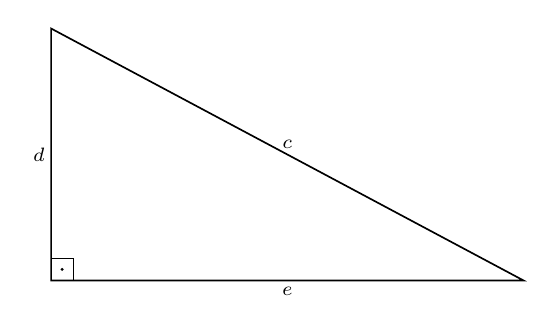
\begin{tikzpicture}[x=1.000cm,y=1.000cm,line width=0.6pt,baseline=(current bounding box.north)]\draw (0.000,0.000) -- (6.000,0.000) -- (0.000,3.200) -- cycle;\draw[line width=0.4pt] (0.280,0.000) -- (0.280,0.280) -- (0.000,0.280);\fill (0.140,0.140) circle (0.6pt);\node[font=\scriptsize,anchor=east,inner sep=2pt] at (0.000,1.600) {$d$};\node[font=\scriptsize,anchor=north,inner sep=2pt] at (3.000,0.000) {$e$};\node[font=\scriptsize,anchor=south,inner sep=2pt] at (3.000,1.600) {$c$};\end{tikzpicture}\par
\rechenplatz{1}
\fusshilfe{\mbox{10:~A = d · e : 2}}
\end{pfaufg}
\pfgruppe{}
\begin{pfaufg}{P10 ’24}{11.}{1 BE}
Ein gleichseitiges Dreieck hat die Seitenlänge a. Kreuze die Formel für seinen Umfang u an:
\pfkreuzzeile{$u=a\cdot a\cdot a$}\pfkreuzzeile{$u=a^3$}\pfkreuzzeile{$u=3\cdot a$}\pfkreuzzeile{$u=\tfrac{a}{3}$}
\fusshilfe{\mbox{11:~u = 3 · a}}
\end{pfaufg}
\pfgruppe{}
\begin{pfaufg}{P10 ’14}{12.}{1 BE}
Die graue Figur ist aus gleich großen Quadraten mit der Seitenlänge a zusammengesetzt. Gib einen Term für ihren Umfang u an.
\par\smallskip\noindent \begin{tikzpicture}[line width=0.6pt,baseline=(current bounding box.north)]\draw[mbgitter,line width=0.3pt,step=0.5] (-0.5,-0.5) grid (3.0,2.0);\fill[black!30,draw=black] (0,0.5) -- (1,0.5) -- (1,0) -- (1.5,0) -- (1.5,0.5) -- (2.5,0.5) -- (2.5,1) -- (1.5,1) -- (1.5,1.5) -- (1,1.5) -- (1,1) -- (0,1) -- cycle;\node[font=\small,anchor=east] at (0,0.75) {$a$};\end{tikzpicture}\par
\rechenplatz{1}
\fusshilfe{\mbox{12:~u = 16a}}
\end{pfaufg}
\pfgruppe{}
\begin{pfaufg}{P10 ’25}{13.}{1 BE}
Die Abbildung zeigt ein Rechteck. Kreuze die Gleichung an, mit der man seinen gesamten Flächeninhalt berechnet:
\pfkreuzzeile{$A=2\cdot(a+b+c)$}\pfkreuzzeile{$A=a+2\cdot a\cdot b$}\pfkreuzzeile{$A=a\cdot(b+c)$}\pfkreuzzeile{$A=a\cdot b\cdot c$}
\par\smallskip\noindent 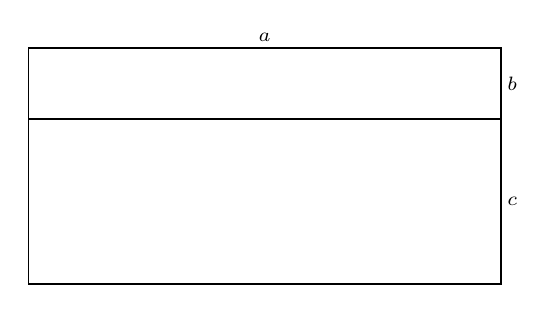
\begin{tikzpicture}[x=1.000cm,y=1.000cm,line width=0.6pt,baseline=(current bounding box.north)]\draw (0.000,0.000) -- (6.000,0.000) -- (6.000,3.000) -- (0.000,3.000) -- cycle;\draw[] (0.000,2.100) -- (6.000,2.100);\node[font=\scriptsize,anchor=south,inner sep=2pt] at (3.000,3.000) {$a$};\node[font=\scriptsize,anchor=west,inner sep=2pt] at (6.000,2.550) {$b$};\node[font=\scriptsize,anchor=west,inner sep=2pt] at (6.000,1.050) {$c$};\end{tikzpicture}\par
\fusshilfe{\mbox{13:~A = a · (b + c)}}
\end{pfaufg}
\pfstufekopf[sgrundfigurberechnen]{Grundfigur berechnen}{in 5 der letzten 5 Prüfungen}
\pfgruppe{}
\begin{pfaufg}{}{14.}{}
Die Figur zeigt ein Parallelogramm mit der Grundseite $g$. Zeichne die Höhe zu $g$ ein und markiere den rechten Winkel.
\par\smallskip\noindent \parallelogramm[seiten={$g$,,,}]{4}{2.5}{60}\par
\rechenplatz{1}
\end{pfaufg}
\begin{pfaufg}{}{15.}{}
Die Figur zeigt ein Viereck. In den Formeln sind $a$ und $c$ parallele Seiten, $h$ ist die Höhe. $e$ und $f$ sind Diagonalen. Kreuze an, welche Formel zur Figur passt. 
\pfkreuzzeile{$A = a \cdot h$}\pfkreuzzeile{$A = \tfrac{a + c}{2} \cdot h$}\pfkreuzzeile{$A = \tfrac{e \cdot f}{2}$}
\par\smallskip\noindent \trapez[hoehe=h]{5}{3}{2.5}\par
\fusshilfe{\mbox{15:~$\tfrac{a + c}{2} \cdot h$}}
\end{pfaufg}
\pfgruppe{}
\begin{pfaufg}{}{16.}{}
Ein Parallelogramm hat die Grundseite $g = 9$ cm und die Höhe $h = 4$ cm. Berechne die Fläche des Parallelogramms.
\par\noindent A = \leerfeld[cm²] \par
\fusshilfe{\mbox{16:~$36$ cm²}}
\end{pfaufg}
\pfgruppe{}
\begin{pfaufg}{}{17.}{}
Ein Trapez hat die parallelen Seiten $a = 9$ cm und $c = 5$ cm. Die Höhe ist $h = 4$ cm. Berechne die Fläche des Trapezes.
\par\noindent A = \leerfeld[cm²] \par
\fusshilfe{\mbox{17:~$28$ cm²}}
\end{pfaufg}
\pfgruppe{}
\begin{pfaufg}{}{18.}{}
Ein Drachenviereck hat die Diagonalen $e = 7$ cm und $f = 6$ cm. Berechne die Fläche des Drachenvierecks.
\par\noindent A = \leerfeld[cm²] \par
\fusshilfe{\mbox{18:~$21$ cm²}}
\end{pfaufg}
\pfgruppe{}
\begin{pfaufg}{P10 ’25}{19.}{2 BE}
Ein Drachenviereck ABCD (A links, D oben, C rechts, B unten) hat die Diagonalen AC = 50 cm und BD = 80 cm. Sie schneiden sich in F im rechten Winkel. Die Strecke DF ist 25 cm lang. Der Winkel bei D heißt $\gamma$. Ein Drachenviereck ABCD hat die Diagonalen AC = 50 cm und BD = 80 cm; sie schneiden sich im rechten Winkel. Ermittle den Flächeninhalt des Drachenvierecks.
\par\smallskip\noindent \begin{tikzpicture}[x=1.000cm,y=1.000cm,line width=0.6pt,baseline=(current bounding box.north)]\draw (0.000,1.750) -- (3.000,0.000) -- (6.000,1.750) -- (3.000,3.500) -- cycle;\draw[] (0.000,1.750) -- (3.000,1.750);\draw[] (3.000,1.750) -- (6.000,1.750);\draw[] (3.000,0.000) -- (3.000,1.750);\draw[] (3.000,1.750) -- (3.000,3.500);\draw[line width=0.4pt] (3.000,1.470) -- (3.280,1.470) -- (3.280,1.750);\fill (3.140,1.610) circle (0.6pt);\node[font=\small,inner sep=1pt] at (3.000,3.800) {$D$};\node[font=\small,inner sep=1pt] at (3.000,-0.300) {$B$};\node[font=\small,inner sep=1pt] at (-0.300,1.750) {$A$};\node[font=\small,inner sep=1pt] at (6.300,1.750) {$C$};\node[font=\small,inner sep=1pt] at (3.000,1.750) {$F$};\node[font=\scriptsize,mbgrau,anchor=north west] at ([yshift=-2pt]current bounding box.south west) {nicht maßstabsgerecht};\end{tikzpicture}\par
\rechenplatz{1}
\fusshilfe{\mbox{19:~2000 cm²}}
\end{pfaufg}
\begin{pfaufg}{BY ’25}{20.}{}
Von vier Vierecken sind Umfang und Flächeninhalt bekannt: (1) u = 20 cm, A = 16 cm²; (2) u = 24 cm, A = 36 cm²; (3) u = 27 cm, A = 81 cm²; (4) u = 72 cm, A = 134 cm². Eines ist ein Quadrat. Kreuze es an.
\par\smallskip\noindent \sachtabelle{l}{vier Vierecke mit u und A}{}\par
\fusshilfe{\mbox{20:~Viereck 2: Seite 6 cm, u = 24 cm, A = 36 cm²}}
\end{pfaufg}
\begin{pfaufg}{BW ’21}{21.}{}
Trage A($-$3 | 3), B(3 | $-$4) und C(1 | 3) ein (1 LE = 1 cm) und verbinde sie. Zeichne die Höhe h\_b. Wie groß ist die Fläche des Dreiecks?
\par\smallskip\noindent \begin{tikzpicture}\begin{axis}[xmin=-4,xmax=4,ymin=-5,ymax=4,axis lines=middle,tick label style={font=\scriptsize},clip=true,/pgf/number format/use comma,axis line style={-{Stealth[length=2mm]}},every axis plot/.append style={line width=0.9pt},x=0.55cm,y=0.55cm,xtick distance=1,ytick distance=1,enlargelimits=false,grid=both,grid style={mbgitter,line width=0.3pt},major grid style={mbgitter},xlabel={$x$},ylabel={$y$},x label style={anchor=west},y label style={anchor=south}]\end{axis}\end{tikzpicture}\par
\rechenplatz{2}
\fusshilfe{\mbox{21:~b = AC = 4 cm; h\_b = 7 cm; A = 14 cm²}}
\end{pfaufg}
\pfgruppe{}
\begin{pfaufg}{}{22.}{}
Die Figur zeigt ein rechtwinkliges Dreieck. Berechne die Fläche des Dreiecks.
\par\smallskip\noindent \dreieckrw{5}{2.67}{$15$ cm}{$8$ cm}{$17$ cm}\par
\par\noindent A = \leerfeld[cm²] \par
\fusshilfe{\mbox{22:~$60$ cm²}}
\end{pfaufg}
\begin{pfaufg}{P10 ’26}{23.}{1 BE}
Ein Rechteck ist a = 3,5 cm lang und b = 1,5 cm breit. Gib seinen Umfang an.
\rechenplatz{1}
\fusshilfe{\mbox{23:~10 cm}}
\end{pfaufg}
\pfgruppe{}
\begin{pfaufg}{P10 ’24}{24.}{2 BE}
Eine Firma stellt Kegel mit dem Radius r = 30 cm und der Höhe h = 80 cm her. Eine Firma stellt Kegel mit dem Radius r = 30 cm und der Höhe h = 80 cm her. Berechne den Flächeninhalt der Grundfläche eines Kegels.
\par\smallskip\noindent \begin{tikzpicture}[line width=0.6pt,baseline=(current bounding box.north)]\fill[black!15] (0,0) ellipse (1.2 and 0.36);\draw (-1.20,0.00) arc (180:360:1.20 and 0.36);\draw[dashed] (1.20,0.00) arc (0:180:1.20 and 0.36);\draw (-1.2,0) -- (0,2.4) -- (1.2,0);\node[font=\scriptsize,mbgrau,anchor=north west] at ([yshift=-2pt]current bounding box.south west) {nicht maßstabsgerecht};\end{tikzpicture}\par
\rechenplatz{1}
\fusshilfe{\mbox{24:~900$\pi$ $\approx$ 2827,4 cm²}, \mbox{Tipp: $G$ = $\pi$ · 30²}}
\end{pfaufg}
\begin{pfaufg}{NI ’24}{25.}{}
Klara will den Rand einer Schultüte (Kreis, r = 12 cm) mit einem 76 cm langen Band bekleben. Reicht das Band? Berechne und entscheide.
\rechenplatz{1}
\fusshilfe{\mbox{25:~u $\approx$ 75,40 cm < 76 cm $\Rightarrow$ reicht}}
\end{pfaufg}
\begin{pfaufg}{}{26.}{}
Ein Kreis hat den Radius $r = 13$ cm. Wie groß ist seine Fläche? Rechne mit der $\pi$-Taste. Runde auf eine Stelle nach dem Komma.
\par\noindent A $\approx$ \leerfeld[cm²] \par
\fusshilfe{\mbox{26:~$\pi \cdot 13^2 \approx 530{,}9$ cm²}}
\end{pfaufg}
\pfgruppe{}
\begin{pfaufg}{P10 ’15}{27.}{3 BE}
Gegeben ist ein Drachenviereck ABCD. Die Diagonale AC ist senkrecht (A unten, C oben), die Diagonale BD waagerecht (D links, B rechts); beide schneiden sich in E im rechten Winkel. Die Seite AD ist 4,1 cm lang. Im Dreieck ABD ist der Winkel bei A 123° und der Winkel bei B 36° groß; der Winkel bei D heißt $\delta$. Im Dreieck AED ist bei E ein rechter Winkel. Die Hypotenuse AD ist 4,1 cm lang, der Winkel bei D beträgt $\delta$ = 21°. Der Flächeninhalt des Dreiecks AED soll berechnet werden. Gib an, welche Seiten und Winkel du dazu brauchst. Schreibe die Rechenschritte in einer sinnvollen Reihenfolge auf.
\par\smallskip\noindent \begin{tikzpicture}[line width=0.6pt,baseline=(current bounding box.north)]\draw (3.40,-1.30) -- (3.40,0.00) -- (0.00,0.00) -- cycle;\node[font=\small,anchor=north] at (3.40,-1.30) {$A$};\node[font=\small,anchor=south west] at (3.40,0.00) {$E$};\node[font=\small,anchor=east] at (0,0) {$D$};\path (0.00,0.00) -- node[font=\scriptsize,below left] {4,1 cm} (3.40,-1.30);\draw[line width=0.4pt] (3.15,0.00) -- (3.15,-0.25) -- (3.40,-0.25);\draw[line width=0.4pt] (1.1,0) arc (0:-20.9:1.1);\node[font=\scriptsize,anchor=west] at (1.15,-0.2) {$\delta = 21°$};\node[font=\scriptsize,mbgrau,anchor=north west] at ([yshift=-2pt]current bounding box.south west) {nicht maßstabsgerecht};\end{tikzpicture}\par
\rechenplatz{1}
\fusshilfe{\mbox{27:~21°, rechter Winkel bei E; ½ · AE · DE}}
\end{pfaufg}
\pfgruppe{}
\begin{pfaufg}{BY ’22}{28.}{}
An einer Hauswand soll ein rechteckiges Gemüsebeet entstehen. Die drei offenen Seiten bekommen einen Zaun von zusammen 12 m Länge. Das Beet soll quadratisch werden. Berechne seinen Flächeninhalt.
\par\smallskip\noindent \fbox{\parbox{0.9\linewidth}{\footnotesize Skizze: Rechteck an einer Hauswand, zwei Seiten x senkrecht zur Wand, eine Seite b parallel, Zaun an drei Seiten}}\par
\rechenplatz{3}
\fusshilfe{\mbox{28:~x = 4 m; A = 16 m²}}
\end{pfaufg}
\begin{pfaufg}{BW ’23}{29.}{}
Von einem achsensymmetrischen Trapez ABCD kennt man A($-$2 | $-$3), B(6 | $-$3) und D(0 | 3). Zeichne die Punkte (1 LE = 1 cm) und bestimme C. Berechne den Flächeninhalt. Sebastian sagt: „Die Gerade y = $-$x + 3 teilt das Trapez in zwei deckungsgleiche Dreiecke.“ Hat er recht?
\par\smallskip\noindent \begin{tikzpicture}\begin{axis}[xmin=-3,xmax=7,ymin=-4,ymax=4,axis lines=middle,tick label style={font=\scriptsize},clip=true,/pgf/number format/use comma,axis line style={-{Stealth[length=2mm]}},every axis plot/.append style={line width=0.9pt},x=0.55cm,y=0.55cm,xtick distance=1,ytick distance=1,enlargelimits=false,grid=both,grid style={mbgitter,line width=0.3pt},major grid style={mbgitter},xlabel={$x$},ylabel={$y$},x label style={anchor=west},y label style={anchor=south}]\end{axis}\end{tikzpicture}\par
\rechenplatz{3}
\fusshilfe{\mbox{29:~C(4; 3); 36 cm²}}
\end{pfaufg}
\pfgruppe{}
\begin{pfaufg}{P10 ’16}{30.}{2 BE}
Beim Kugelstoßen steht man in einem Abwurfring; das ist ein Kreis mit 2,14 m Durchmesser. Ermittle den Flächeninhalt dieses Kreises.
\rechenplatz{2}
\fusshilfe{\mbox{30:~1,1449$\pi$ $\approx$ 3,60 m²}}
\end{pfaufg}
\pfgruppe{}
\begin{pfaufg}{P10 ’15}{31.}{4 BE}
Mia baut das Modell einer Pyramide mit quadratischer Grundfläche: Die Grundkante ist 0,80 m lang, die Pyramide ist 0,68 m hoch. Die Seitenflächen sägt sie aus dünnem Sperrholz. Weise nach, dass sie für eine Seitenfläche etwa 0,32 m² Sperrholz braucht.
\rechenplatz{3}
\fusshilfe{\mbox{31:~$\approx$ 0,32 m²}}
\end{pfaufg}
\pfgruppe{}
\begin{pfaufg}{P10 ’19}{32.}{4 BE}
Auf einem Mast sitzt ein Prisma, dessen Grund- und Deckfläche gleichseitige Dreiecke mit 1,50 m Seitenlänge sind; die Höhe dieser Dreiecke beträgt 1,30 m. Das Prisma ist 1,20 m hoch. Ermittle den Flächeninhalt der Deckfläche. Durch ein Loch ist Regenwasser in das Prisma gelaufen. Zeige mit einer Rechnung, dass etwa 1,2 m³ Wasser hineinpassen. Leer wiegt das Prisma 200 kg; 1 m³ Regenwasser wiegt 1 000 kg. Berechne, wie schwer das Prisma ist, wenn ein Zehntel seines Innenraums (10 \%) voll Wasser ist.
\par\smallskip\noindent \begin{tikzpicture}[line width=0.6pt,baseline=(current bounding box.north)]\draw[fill=black!20] (0,0) -- (3,0) -- (1.5,2.6) -- cycle;\draw[dashed] (1.5,2.6) -- (1.5,0);\draw[line width=0.4pt] (1.75,0.00) -- (1.75,0.25) -- (1.50,0.25);\node[font=\scriptsize,anchor=west] at (1.5,1.2) {$h_{\text{Deckfläche}}$};\node[font=\scriptsize,mbgrau,anchor=north west] at ([yshift=-2pt]current bounding box.south west) {nicht maßstabsgerecht};\end{tikzpicture}\par
\rechenplatz{4}
\fusshilfe{\mbox{32:~0,975 m²; $\approx$ 1,2 m³; $\approx$ 320 kg}}
\end{pfaufg}
\pfsteckt{steckt auch in Nr. 64 (P10 ’17); Nr. 63 (P10 ’18); Nr. 65 (P10 ’22); Nr. 68 (P10 ’23)}
\pfstufekopf[srckwrtsseiteausflche]{rückwärts: Seite aus Fläche}{in 1 der letzten 5 Prüfungen}
\pfgruppe{}
\begin{pfaufg}{}{33.}{}
Du willst wissen, wie viel Farbe man für ein rundes Schild braucht. Kreuze die Formel an, die du brauchst.
\pfkreuzzeile{$u = \pi \cdot d$}\pfkreuzzeile{$A = \pi \cdot r^2$}
\fusshilfe{\mbox{33:~$\pi \cdot r^2$}}
\end{pfaufg}
\begin{pfaufg}{}{34.}{}
Im Bild ist eine Strecke im Kreis beschriftet. Ist sie ein Radius oder ein Durchmesser? Gib auch die andere Länge an.
\par\smallskip\noindent \begin{kreis}[2] \mittelpunkt{M} \durchmesser{20}{$9$ cm} \end{kreis}\par
\par\noindent Die Strecke ist ein \leerfeld[.]  Die andere Länge: \leerfeld \par
\fusshilfe{\mbox{34:~$4{,}5$ cm}}
\end{pfaufg}
\pfgruppe{}
\begin{pfaufg}{}{35.}{}
Ein Quadrat hat die Fläche $A = 64$ cm². Wie lang ist eine Seite des Quadrats?
\par\noindent a = \leerfeld[cm] \par
\fusshilfe{\mbox{35:~$8$ cm}}
\end{pfaufg}
\begin{pfaufg}{}{36.}{}
Eine Raute hat die Fläche $A = 54$ m². Eine Diagonale ist $e = 9$ m lang. Wie lang ist die andere Diagonale $f$?
\par\noindent f = \leerfeld[m] \par
\fusshilfe{\mbox{36:~$12$ m}}
\end{pfaufg}
\begin{pfaufg}{P10 ’20}{37.}{1 BE}
Ein Quadrat hat den Flächeninhalt 36 cm². Gib seine Seitenlänge an.
\rechenplatz{1}
\fusshilfe{\mbox{37:~6 cm}}
\end{pfaufg}
\begin{pfaufg}{P10 ’23}{38.}{1 BE}
Ein Rechteck ist 400 mm breit und hat den Flächeninhalt 42 000 mm². Gib seine Länge an.
\rechenplatz{1}
\fusshilfe{\mbox{38:~105 mm}}
\end{pfaufg}
\pfgruppe{}
\begin{pfaufg}{}{39.}{}
Ein Parallelogramm hat die Fläche $A = 63$ cm² und die Grundseite $g = 9$ cm. Wie lang ist die Höhe des Parallelogramms?
\par\noindent h = \leerfeld[cm] \par
\fusshilfe{\mbox{39:~$7$ cm}}
\end{pfaufg}
\begin{pfaufg}{}{40.}{}
Ein Trapez hat die Fläche $A = 42$ cm². Die parallelen Seiten sind $a = 9$ cm und $c = 5$ cm. Wie lang ist die Höhe des Trapezes?
\par\noindent h = \leerfeld[cm] \par
\fusshilfe{\mbox{40:~$6$ cm}}
\end{pfaufg}
\pfgruppe{}
\begin{pfaufg}{P10 ’18}{41.}{1 BE}
Ein Rechteck hat den Umfang u = 26 cm; die Seite a ist 8 cm lang. Gib die Länge der Seite b an.
\par\smallskip\noindent \begin{tikzpicture}[x=1.000cm,y=1.000cm,line width=0.6pt,baseline=(current bounding box.north)]\draw (0.000,0.000) -- (6.000,0.000) -- (6.000,3.000) -- (0.000,3.000) -- cycle;\node[font=\scriptsize,anchor=north,inner sep=2pt] at (3.000,0.000) {a = 8 cm};\node[font=\scriptsize,anchor=west,inner sep=2pt] at (6.000,1.500) {$b$};\node[font=\scriptsize,mbgrau,anchor=north west] at ([yshift=-2pt]current bounding box.south west) {nicht maßstabsgerecht};\end{tikzpicture}\par
\rechenplatz{2}
\fusshilfe{\mbox{41:~b = 5 cm}}
\end{pfaufg}
\pfgruppe{}
\begin{pfaufg}{P10 ’20}{42.}{2 BE}
Im Dreieck ABC ist bei C ein rechter Winkel; BC ist 12 m und AC 34 m lang. Der Punkt Q liegt auf AC. Das Dreieck QBC hat den Flächeninhalt 90 m². Berechne die Länge der Strecke QC.
\par\smallskip\noindent \begin{tikzpicture}[x=1.000cm,y=1.000cm,line width=0.6pt,baseline=(current bounding box.north)]\draw (0.000,3.500) -- (6.000,3.500) -- (0.000,0.000) -- cycle;\draw[dashed] (0.000,2.800) -- (6.000,3.500);\draw[line width=0.4pt] (0.000,3.220) -- (0.280,3.220) -- (0.280,3.500);\fill (0.140,3.360) circle (0.6pt);\node[font=\small,inner sep=1pt] at (-0.259,3.651) {$C$};\node[font=\small,inner sep=1pt] at (6.288,3.584) {$B$};\node[font=\small,inner sep=1pt] at (-0.195,-0.228) {$A$};\node[font=\small,inner sep=1pt] at (-0.292,2.868) {$Q$};\fill (0.000,2.800) circle (1.4pt);\node[font=\scriptsize,mbgrau,anchor=north west] at ([yshift=-2pt]current bounding box.south west) {nicht maßstabsgerecht};\end{tikzpicture}\par
\rechenplatz{2}
\fusshilfe{\mbox{42:~QC = 15 m}}
\end{pfaufg}
\pfgruppe{}
\begin{pfaufg}{P10 ’14}{43.}{2 BE}
Für ein Café wird eine Kühlvitrine in Form eines Prismas gebaut. Die Grundfläche ist ein gleichschenkliges Trapez mit den parallelen Seiten 110 cm und 80 cm, den Schenkeln 57 cm und dem Flächeninhalt 5 225 cm². Die Vitrine ist 165 cm hoch. Die Rückwand derselben Vitrine ist ein Rechteck, 110 cm breit und 165 cm hoch. Sie soll aus einer rechteckigen Platte gesägt werden, die 1,20 m breit ist und einen Flächeninhalt von 1,8 m² hat. Entscheide mit einer Rechnung, ob die Platte dafür reicht.
\par\smallskip\noindent \begin{tikzpicture}[line width=0.6pt,baseline=(current bounding box.north)]\draw (-1.50,3.70) -- (1.50,3.70) -- (1.09,2.80) -- (-1.09,2.80) -- cycle;\draw (1.50,0.90) -- (1.09,0.00) -- (-1.09,0.00) -- (-1.50,0.90);\draw[dashed] (-1.50,0.90) -- (1.50,0.90);\draw[dashed] (-1.50,0.90) -- (-1.50,3.70);\draw (1.50,0.90) -- (1.50,3.70);\draw (1.09,0.00) -- (1.09,2.80);\draw (-1.09,0.00) -- (-1.09,2.80);\path (-1.50,3.70) -- node[font=\scriptsize,above] {110} (1.50,3.70);\path (-1.09,0.00) -- node[font=\scriptsize,below] {80} (1.09,0.00);\path (1.09,2.80) -- node[font=\scriptsize,right] {57} (1.50,3.70);\path (1.09,0.00) -- node[font=\scriptsize,right] {165} (1.09,2.80);\node[font=\scriptsize,mbgrau,anchor=north west] at (-2,-0.4) {Maße in cm};\node[font=\scriptsize,mbgrau,anchor=north west] at ([yshift=-2pt]current bounding box.south west) {nicht maßstabsgerecht};\end{tikzpicture}\par
\rechenplatz{2}
\fusshilfe{\mbox{43:~nein, Plattenlänge 1,5 m < 1,65 m}}
\end{pfaufg}
\pfgruppe{}
\begin{pfaufg}{P10 ’14}{\llap{\textasteriskcentered\,}44.}{3 BE}
Für ein Café wird eine Kühlvitrine in Form eines Prismas gebaut. Die Grundfläche ist ein gleichschenkliges Trapez mit den parallelen Seiten 110 cm und 80 cm, den Schenkeln 57 cm und dem Flächeninhalt 5 225 cm². Die Vitrine ist 165 cm hoch. Eine Kühlvitrine hat die Form eines Prismas. Ihre Grundfläche ist ein gleichschenkliges Trapez mit den parallelen Seiten 110 cm und 80 cm und dem Flächeninhalt 5 225 cm². Die Höhe h dieses Trapezes ist die Tiefe der Vitrine. Weise nach, dass Kuchenplatten mit 50 cm Durchmesser in die Vitrine passen.
\par\smallskip\noindent \begin{tikzpicture}[x=1.000cm,y=1.000cm,line width=0.6pt,baseline=(current bounding box.north)]\draw (0.818,0.000) -- (5.182,0.000) -- (6.000,3.000) -- (0.000,3.000) -- cycle;\draw[dashed] (0.818,3.000) -- (0.818,0.000);\draw[line width=0.4pt] (1.098,0.000) -- (1.098,0.280) -- (0.818,0.280);\fill (0.958,0.140) circle (0.6pt);\node[font=\scriptsize,anchor=north,inner sep=2pt] at (3.000,0.000) {80 cm};\node[font=\scriptsize,anchor=south,inner sep=2pt] at (3.000,3.000) {110 cm};\node[font=\scriptsize,anchor=west,inner sep=2pt] at (5.591,1.500) {57 cm};\node[font=\scriptsize,anchor=east,inner sep=2pt] at (0.818,1.500) {$h$};\node[font=\scriptsize,mbgrau,anchor=north west] at ([yshift=-2pt]current bounding box.south west) {nicht maßstabsgerecht};\end{tikzpicture}\par
\rechenplatz{2}
\fusshilfe{\mbox{44:~55 cm > 50 cm $\Rightarrow$ Tiefe reicht}}
\end{pfaufg}
\pfstufekopf[sfigurerstzerlegenode]{Figur erst zerlegen oder Strecke erst berechnen}{in 3 der letzten 5 Prüfungen}
\pfgruppe{}
\begin{pfaufg}{}{45.}{}
Die Figur zeigt ein Viereck. Schreibe auf, in welche einfachen Teilflächen du es zerlegen kannst.
\par\smallskip\noindent \viereck{(0,0)}{(6,0)}{(6,3)}{(2,3)}\par
\rechenplatz{1}
\fusshilfe{\mbox{45:~ein Rechteck und ein rechtwinkliges Dreieck}}
\end{pfaufg}
\begin{pfaufg}{}{46.}{}
Im Bild ist ein Teil des Kreises grau. Kreuze an, welcher Teil des Kreises das ist.
\pfkreuzzeile{$\tfrac{1}{2}$}\pfkreuzzeile{$\tfrac{1}{3}$}\pfkreuzzeile{$\tfrac{1}{4}$}
\par\smallskip\noindent \kreissektor{180}{}\par
\fusshilfe{\mbox{46:~$\tfrac{1}{2}$}}
\end{pfaufg}
\pfgruppe{}
\begin{pfaufg}{}{47.}{}
Ein Beet hat die Form eines L. Es besteht aus zwei Rechtecken. Das erste Rechteck hat die Seiten $8$ m und $3$ m. Das zweite hat die Seiten $3$ m und $4$ m. Berechne die Fläche des Beets.
\par\noindent A = \leerfeld[m²] \par
\fusshilfe{\mbox{47:~$36$ m²}}
\end{pfaufg}
\begin{pfaufg}{}{48.}{}
Ein Kreisausschnitt hat den Mittelpunktswinkel $\alpha = 90^\circ$. Welcher Teil des Kreises ist das? Gib den Anteil als Bruch an.
\par\noindent \leerfeld \par
\fusshilfe{\mbox{48:~$\tfrac{1}{4}$}}
\end{pfaufg}
\begin{pfaufg}{}{49.}{}
Eine Holzplatte hat die Seiten $70$ cm und $45$ cm. Aus ihr wird ein Quadrat mit $15$ cm Seitenlänge ausgesägt. Berechne die Fläche der übrigen Platte.
\par\noindent A = \leerfeld[cm²] \par
\fusshilfe{\mbox{49:~$2\,925$ cm²}}
\end{pfaufg}
\begin{pfaufg}{}{50.}{}
Ein Rechteck hat die Seiten $11$ m und $6$ m. An einer Ecke fehlt ein kleines Rechteck mit den Seiten $5$ m und $2$ m. Berechne den Umfang der übrigen Figur.
\par\noindent u = \leerfeld[m] \par
\fusshilfe{\mbox{50:~die fehlende Ecke ändert den Umfang nicht}}
\end{pfaufg}
\begin{pfaufg}{P10 ’17}{51.}{2 BE}
Familie Sommer hat einen Swimmingpool gebaut. Seine Grundfläche ist ein Rechteck, an dessen kurze Seiten je ein Halbkreis angesetzt ist. Die kurze Seite des Rechtecks ist a = 5 m lang, die lange Seite b = 10 m. Gib an, aus welchen Teilflächen die Grundfläche des Pools besteht.
\par\smallskip\noindent \begin{tikzpicture}[line width=0.6pt,baseline=(current bounding box.north)]\begin{scope}\clip (0,0) -- (3.0,0) arc (-90:90:0.9) -- (0,1.8) arc (90:270:0.9) -- cycle;\foreach \i in {-30,...,30}{\draw[line width=0.3pt] (\i*0.2-3,-3) -- ++(7,7);}\end{scope}\draw (0,0) -- (3.0,0) arc (-90:90:0.9) -- (0,1.8) arc (90:270:0.9) -- cycle;\draw[dashed] (0,0) -- (0,1.8);\node[font=\scriptsize,left,fill=white,inner sep=1pt] at (-0.9500000000000001,0.9) {$a$ = 5 m};\node[font=\scriptsize,below] at (1.5,0) {$b$ = 10 m};\node[font=\scriptsize,mbgrau,anchor=north west] at ([yshift=-2pt]current bounding box.south west) {nicht maßstabsgerecht};\end{tikzpicture}\par
\rechenplatz{1}
\fusshilfe{\mbox{51:~Rechteck 10 m × 5 m und zwei Halbkreise}}
\end{pfaufg}
\pfgruppe{}
\begin{pfaufg}{P10 ’25}{52.}{2 BE}
Bestimme, wie viel Prozent der Kreisfläche grau gefärbt sind.
\par\smallskip\noindent \begin{tikzpicture}[line width=0.6pt,baseline=(current bounding box.north)]\draw (0,0) circle (1.5); \fill[black!25] (0,0) -- (90:1.5) arc (90:-55:1.5) -- cycle;\draw (0,0) -- (90:1.5); \draw (0,0) -- (-55:1.5); \fill (0,0) circle (1.3pt);\node[font=\small] at (17.5:0.9) {145°};\draw[line width=0.4pt] (0.00,0.00) ++(90:0.35) arc (90:305:0.35);\node[font=\scriptsize,fill=white,inner sep=0.5pt] at ($(0.00,0.00)+(197.5:0.6499999999999999)$) {$\alpha$};\node[font=\scriptsize,mbgrau,anchor=north west] at ([yshift=-2pt]current bounding box.south west) {nicht maßstabsgerecht};\end{tikzpicture}\par
\rechenplatz{1}
\fusshilfe{\mbox{52:~$\tfrac{29}{72}$ $\approx$ 40,3 \%}}
\end{pfaufg}
\pfgruppe{}
\begin{pfaufg}{nach HH ’26}{53.}{}
Ein regelmäßiges Sechseck besteht aus sechs gleichseitigen Dreiecken mit 9 cm Seitenlänge und 7,8 cm Höhe. Bestätige, dass seine Fläche etwa 210 cm² beträgt.
\par\smallskip\noindent \fbox{\parbox{0.9\linewidth}{\footnotesize Skizze: Sechseck, in sechs Dreiecke zerlegt}}\par
\rechenplatz{1}
\fusshilfe{\mbox{53:~A = 6 · ½ · 9 · 7,79 $\approx$ 210 cm²}}
\end{pfaufg}
\begin{pfaufg}{}{54.}{}
Eine quadratische Tischplatte hat $90$ cm Seitenlänge. In der Mitte hat sie ein rundes Loch für den Sonnenschirm. Das Loch hat den Radius $r = 5$ cm. Berechne die Fläche der Platte ohne das Loch. Runde auf ganze cm².
\par\noindent A = \leerfeld[cm²] \par
\fusshilfe{\mbox{54:~$90 \cdot 90 - \pi \cdot 5^2 \approx 8\,021$ cm²}}
\end{pfaufg}
\begin{pfaufg}{}{55.}{}
Ein Kreisring hat außen den Radius $7$ cm und innen den Radius $4$ cm. Wie groß ist seine Fläche? Rechne mit der $\pi$-Taste. Runde auf eine Stelle nach dem Komma.
\par\noindent A $\approx$ \leerfeld[cm²] \par
\fusshilfe{\mbox{55:~$\pi \cdot 7^2 - \pi \cdot 4^2 \approx 103{,}7$ cm²}}
\end{pfaufg}
\pfgruppe{}
\begin{pfaufg}{}{56.}{}
Ein gleichschenkliges Trapez hat die parallelen Seiten $a = 14$ cm und $c = 8$ cm. Die Höhe ist $h = 4$ cm. Berechne den Umfang des Trapezes.
\par\noindent u = \leerfeld[cm] \par
\fusshilfe{\mbox{56:~$32$ cm}}
\end{pfaufg}
\begin{pfaufg}{BY ’23}{57.}{}
Ein Quadrat mit 8 cm Seitenlänge wird in zwei Rechtecke geteilt. Das größere Rechteck hat einen Umfang von 28 cm. Wie groß ist der Umfang des kleineren? Kreuze an: 12 cm; 16 cm; 20 cm; 22 cm; 26 cm.
\par\smallskip\noindent \fbox{\parbox{0.9\linewidth}{\footnotesize Skizze: Quadrat 8 cm × 8 cm, durch eine Linie in zwei Rechtecke geteilt}}\par
\rechenplatz{3}
\fusshilfe{\mbox{57:~Umfang 20 cm}}
\end{pfaufg}
\pfgruppe{}
\begin{pfaufg}{nach BW ’21}{58.}{}
Ein Dach hat die Form eines regelmäßigen Achtecks. Es besteht aus 8 gleichen Dreiecken. Jedes hat die Grundseite 2 m und die Höhe 2,41 m. Berechne die Dachfläche.
\par\smallskip\noindent \fbox{\parbox{0.9\linewidth}{\footnotesize Skizze: Achteck in 8 Dreiecke vom Mittelpunkt aus zerlegt; ein Dreieck mit g = 2 m, h = 2,41 m}}\par
\rechenplatz{2}
\fusshilfe{\mbox{58:~19,28 m²}}
\end{pfaufg}
\begin{pfaufg}{BY ’25}{59.}{}
Im Trapez ABCD sind die parallelen Seiten AB = 12 cm und CD = 6,57 cm lang. Die Diagonale BD ist 14,10 cm lang und bildet mit AB einen Winkel von 40°. Berechne die Höhe DE und den Flächeninhalt des Trapezes.
\par\smallskip\noindent \fbox{\parbox{0.9\linewidth}{\footnotesize Skizze: Trapez ABCD mit Diagonale BD und Höhe DE}}\par
\rechenplatz{2}
\fusshilfe{\mbox{59:~$\approx$ 9,06 cm; $\approx$ 84,12 cm²}}
\end{pfaufg}
\begin{pfaufg}{NI ’26}{60.}{}
Die Öffnung einer Taschentuchbox besteht aus einem Rechteck (13 cm × 5 cm) und zwei Halbkreisen mit 5 cm Durchmesser an den kurzen Seiten. Berechne ihren Flächeninhalt.
\par\smallskip\noindent \fbox{\parbox{0.9\linewidth}{\footnotesize Skizze: Langloch aus Rechteck 13 cm × 5 cm und zwei Halbkreisen (d = 5 cm); nicht maßstäblich}}\par
\rechenplatz{2}
\fusshilfe{\mbox{60:~$\approx$ 84,63 cm²}}
\end{pfaufg}
\begin{pfaufg}{BW ’23}{61.}{}
In einem Zimmer soll neuer Boden verlegt werden. Zerlege den Grundriss in zwei Trapeze und zwei Rechtecke und berechne die Fläche.
\par\smallskip\noindent \fbox{\parbox{0.9\linewidth}{\footnotesize Skizze: Grundriss (in cm, Maßstab des Plans) aus Trapez mit a = 5, c = 3, h = 2; Trapez mit a = 5, c = 2, h = 1,5; zwei Rechtecke je 5 × 0,5}}\par
\rechenplatz{3}
\fusshilfe{\mbox{61:~18,25 (8 + 5,25 + 2 · 2,5) Flächeneinheiten}}
\end{pfaufg}
\begin{pfaufg}{BY ’23}{62.}{}
Das Trapez ABCD ist gleichschenklig. DE ist seine Höhe, E liegt auf AB. Es gilt: AB = 11 cm, AE = 4 cm und $\angle$BAD = 60°. Berechne die Längen DE und DC. Zeige, dass das Trapez den Flächeninhalt 28√3 cm² hat.
\par\smallskip\noindent \fbox{\parbox{0.9\linewidth}{\footnotesize Skizze: gleichschenkliges Trapez ABCD mit AB unten, Höhe DE, Winkel 60° bei A}}\par
\rechenplatz{3}
\fusshilfe{\mbox{62:~4√3 cm $\approx$ 6,93 cm; 3 cm; 28√3 cm² $\approx$ 48,50 cm²}}
\end{pfaufg}
\begin{pfaufg}{P10 ’18}{63.}{3 BE}
Ein runder Turm mit 6,4 m Durchmesser steht auf einer Rasenfläche, die 20,0 m × 12,0 m groß ist. Der Rasen um den Turm herum soll neu angelegt werden. Berechne die Fläche des neuen Rasens.
\par\smallskip\noindent \begin{tikzpicture}[line width=0.6pt,baseline=(current bounding box.north)]\draw[dotted,line width=0.9pt] (0,0) rectangle (3.6,2.4);\draw[fill=black!20] (1.8,1.2) circle (1.0);\node[font=\scriptsize,mbgrau,anchor=north west] at ([yshift=-2pt]current bounding box.south west) {nicht maßstabsgerecht};\end{tikzpicture}\par
\rechenplatz{3}
\fusshilfe{\mbox{63:~240 $-$ 10,24$\pi$ $\approx$ 207,83 m²}}
\end{pfaufg}
\begin{pfaufg}{P10 ’17}{64.}{3 BE}
Familie Sommer hat einen Swimmingpool gebaut. Seine Grundfläche ist ein Rechteck, an dessen kurze Seiten je ein Halbkreis angesetzt ist. Die kurze Seite des Rechtecks ist a = 5 m lang, die lange Seite b = 10 m. Berechne den Flächeninhalt der Grundfläche des Pools.
\par\smallskip\noindent \begin{tikzpicture}[line width=0.6pt,baseline=(current bounding box.north)]\begin{scope}\clip (0,0) -- (3.0,0) arc (-90:90:0.9) -- (0,1.8) arc (90:270:0.9) -- cycle;\foreach \i in {-30,...,30}{\draw[line width=0.3pt] (\i*0.2-3,-3) -- ++(7,7);}\end{scope}\draw (0,0) -- (3.0,0) arc (-90:90:0.9) -- (0,1.8) arc (90:270:0.9) -- cycle;\draw[dashed] (0,0) -- (0,1.8);\node[font=\scriptsize,left,fill=white,inner sep=1pt] at (-0.9500000000000001,0.9) {$a$ = 5 m};\node[font=\scriptsize,below] at (1.5,0) {$b$ = 10 m};\node[font=\scriptsize,mbgrau,anchor=north west] at ([yshift=-2pt]current bounding box.south west) {nicht maßstabsgerecht};\end{tikzpicture}\par
\rechenplatz{3}
\fusshilfe{\mbox{64:~50 + 6,25$\pi$ $\approx$ 69,63 m²}}
\end{pfaufg}
\pfgruppe{}
\begin{pfaufg}{P10 ’22}{\llap{\textasteriskcentered\,}65.}{3 BE}
Gegeben ist ein Dreieck ABC, das nicht rechtwinklig ist. Die Höhe $h_c$ von C auf die Seite AB ist etwa 7,4 m lang; ihr Fußpunkt heißt D. Die Seite b = AC ist 14,1 m lang, der Winkel bei B ist 52° groß. Der Winkel bei C zwischen AC und der Höhe heißt $\gamma_1$. Im Dreieck ABC ist die Höhe $h_c$ $\approx$ 7,4 m; ihr Fußpunkt D liegt auf AB. Der Winkel bei B beträgt 52°. Gegeben: AD $\approx$ 12,0 m. Ermittle den Flächeninhalt des Dreiecks ABC.
\par\smallskip\noindent \begin{tikzpicture}[x=1.000cm,y=1.000cm,line width=0.6pt,baseline=(current bounding box.north)]\draw (0.000,0.000) -- (6.000,0.000) -- (3.000,3.500) -- cycle;\draw[dashed] (3.000,3.500) -- (3.000,0.000);\draw[line width=0.4pt] (3.000,0.280) -- (2.720,0.280) -- (2.720,0.000);\fill (2.860,0.140) circle (0.6pt);\draw[line width=0.4pt] (5.727,0.319) arc (130.60:180.00:0.420);\node[font=\scriptsize,inner sep=0.5pt,fill=white] at (5.164,0.384) {52°};\node[font=\scriptsize,anchor=west,inner sep=2pt] at (3.000,1.750) {$h_c$};\node[font=\scriptsize,anchor=east,inner sep=2pt] at (1.500,1.750) {b = 14,1 m};\node[font=\small,inner sep=1pt] at (-0.280,-0.109) {$A$};\node[font=\small,inner sep=1pt] at (6.280,-0.109) {$B$};\node[font=\small,inner sep=1pt] at (3.000,3.800) {$C$};\node[font=\small,inner sep=1pt] at (3.000,-0.300) {$D$};\node[font=\scriptsize,mbgrau,anchor=north west] at ([yshift=-2pt]current bounding box.south west) {nicht maßstabsgerecht};\end{tikzpicture}\par
\rechenplatz{3}
\fusshilfe{\mbox{65:~A = 3,7 · (√144,05 + 7,4 : tan 52°) $\approx$ 65,8 m²}}
\end{pfaufg}

\pfstufekopf[santeilinprozentversc]{Anteil in Prozent (Verschnitt)}{in 1 der letzten 5 Prüfungen}
\pfgruppe{}
\begin{pfaufg}{}{66.}{}
Für ein Buntglasfenster wird aus einer rechteckigen Glasscheibe ein Trapez geschnitten. Die Scheibe ist $50$ cm lang und $30$ cm breit. Die parallelen Seiten des Trapezes sind $50$ cm und $34$ cm lang, seine Höhe ist $30$ cm. Der Rest der Scheibe ist Abfall. Wie viel Prozent der Scheibe sind Abfall?
\rechenplatz{4}
\fusshilfe{\mbox{66:~$16\,\%$}}
\end{pfaufg}
\pfgruppe{}
\begin{pfaufg}{NI ’22}{67.}{}
Simone schneidet eine runde Tischdecke mit 115 cm Durchmesser aus einem Stoffrechteck von 15 000 cm². Der Rest ist Verschnitt. Berechne den Verschnitt in Prozent.
\rechenplatz{3}
\fusshilfe{\mbox{67:~$\approx$ 10 386,89 cm²; $\approx$ 30,75 \%}}
\end{pfaufg}
\pfgruppe{}
\begin{pfaufg}{P10 ’23}{\llap{\textasteriskcentered\,}68.}{4 BE}
Eine Konservendose hat die Form eines Zylinders mit dem Radius 4 cm und der Höhe 8 cm. Für Konservendosen werden kreisrunde Deckel mit dem Radius 4 cm aus Blechstreifen ausgestanzt, die 8 cm breit und 1 m lang sind. Aus jedem Streifen sollen möglichst viele Deckel entstehen. Der Abfall darf höchstens 25 \% eines Streifens ausmachen. Überprüfe rechnerisch, ob diese Vorgabe eingehalten wird.
\rechenplatz{4}
\fusshilfe{\mbox{68:~$\approx$ 24,6 \% $\le$ 25 \%}}
\end{pfaufg}
\pfpruefstein{P10 ’23}
\begin{pfaufg}{}{}{}
Gegeben ist ein Trapez mit den parallelen Seiten 25,80 m (unten) und 15,00 m (oben). Es ist 8,00 m hoch. Die beiden Winkel an der unteren Seite sind je 56° groß.
\par\smallskip\noindent \begin{tikzpicture}[x=1.000cm,y=1.000cm,line width=0.6pt,baseline=(current bounding box.north)]\draw (0.000,0.000) -- (6.000,0.000) -- (4.744,1.860) -- (1.256,1.860) -- cycle;\draw[dashed] (1.256,1.860) -- (1.256,0.000);\draw[line width=0.4pt] (1.536,0.000) -- (1.536,0.280) -- (1.256,0.280);\fill (1.396,0.140) circle (0.6pt);\draw[line width=0.4pt] (0.420,0.000) arc (0.00:55.98:0.420);\node[font=\scriptsize,inner sep=0.5pt,fill=white] at (0.812,0.432) {56°};\draw[line width=0.4pt] (5.765,0.348) arc (124.02:180.00:0.420);\node[font=\scriptsize,inner sep=0.5pt,fill=white] at (5.188,0.432) {56°};\draw[line width=0.4pt] (4.324,1.860) arc (180.00:304.02:0.420);\node[font=\scriptsize,inner sep=0.5pt,fill=white] at (4.397,1.207) {$\gamma$};\node[font=\scriptsize,anchor=north,inner sep=2pt] at (3.000,0.000) {25,80 m};\node[font=\scriptsize,anchor=south,inner sep=2pt] at (3.000,1.860) {15,00 m};\node[font=\scriptsize,anchor=east,inner sep=2pt] at (1.256,0.930) {8,00 m};\node[font=\scriptsize,mbgrau,anchor=north west] at ([yshift=-2pt]current bounding box.south west) {nicht maßstabsgerecht};\end{tikzpicture}\par
\end{pfaufg}
\begin{pfaufg}{}{a)}{1 BE}
Ein Trapez hat die parallelen Seiten 25,80 m (unten) und 15,00 m (oben) und ist 8,00 m hoch. Die beiden Winkel an der unteren Seite sind je 56° groß. Gib die Größe des Winkels $\gamma$ oben rechts an.
\rechenplatz{3}
\fusshilfe{\mbox{Prüfstein a):~$\gamma$ = 124°}}
\end{pfaufg}
\begin{pfaufg}{}{b)}{2 BE}
Berechne den Flächeninhalt des Trapezes.
\rechenplatz{3}
\fusshilfe{\mbox{Prüfstein b):~A = 163,2 m²}}
\end{pfaufg}
\begin{pfaufg}{}{*c)}{3 BE}
Berechne den Umfang des Trapezes.
\rechenplatz{3}
\fusshilfe{\mbox{Prüfstein c):~U = 40,8 + 16 : sin 56° $\approx$ 60,1 m}}
\end{pfaufg}
\end{document}